\documentclass[12pt]{article}
\usepackage[onehalfspacing]{setspace}
\usepackage[ngerman]{babel}
\usepackage{graphicx}
\graphicspath{ {./images/} }

\begin{document}
	
\title{Zelluläre Automaten}
\author{Carl Heinrich Bellgardt}	
	
\section{Zelluläre Automaten}
\subsection{Definition}
	\glqq Zellularautomaten sind dynamsische mathematische Systeme, die durch eine rekursive Folge diskreter Systemzustände gebildet werden. Die Zellularautomaten bestehen typischerweise aus einer Menge von Elementen mit definierten Zuständen, Zellen genannt, die in einem ein- oder mehrdimensionalen Gitter angeordnet und durch lokale Interaktionsregeln mit den Zellen in einer definierter Nachbarschaft verknüpft sind\footnote{Schmidt, 2014, S. 1}.\grqq{} Beim betreiben des Automaten, meistens in programmierter Form, wird dann bei jedem Schritt, oft Tick genannt, für jede Zelle die lokale Überführungsfunktion angewendet, welche als Eingaben den Zustand der Zelle und aller Zellen in ihrer Nachbarschaft verwendet. Daraus ergibt sich dann der neue Zustand der Zelle. Sobald dies für jede Zelle im Raum geschehen ist, endet der Schritt.
\subsection{Was wird dabei beobachtet?}
	Beobachtet wird bei diesen Versuchen meist die Entwicklung innerhalb eines Zeitraumes, als eine Anzahl von Ticks, in Abhängigkeit von den Startwerten. Nicht nur die Werte, durch die sich der Zellautomat definiert, sind dabei entscheidend, auch das Aussehen des Raumes vor dem ersten Tick spielt eine große Rolle.
\subsection{Darstellung der Ergebnisse}
	Bei einem eindimensionalen Zellautomaten wird jeder Tick in einer neuen Zeile dargestellt. Die Y-Achse zeigt somit den Verlauf mit jedem Tick, sie ist die Zeit-Achse. Bei einem zweidimensionalen Zellautomaten hingegen erhält man mit jedem Tick eine zweidimensionale Ausgabe, was bedeutet, dass die Ausgabe von einem Zeitraum aus Ticks dreidimensional ist. Um diese Daten zu visualisieren, zeigt man darum alle Ticks einzeln hintereinander, wie ein Video.

\newpage

\section{Der bekannteste zelluläre Automat}
\subsection{Game of Life}
	Der wohl bekannteste zelluläre Automat, \glqq John Conway's Game of Life\grqq{}\footnote{auf Deutsch: \glqq Spiel des Lebens\grqq{}}, ist ein zweidimensionaler Automat, der gerne von angehenden Informatikern als Programmieraufgabe umgesetzt wird.
	Die Berechnung ist zwar nicht sehr komplex, jedoch erreicht man eine Vielzahl an Phänomenen, die es zu beobachten, notieren und analysieren gilt.
\subsection{Die Regeln}
	\glqq 1968 war John Conway ein junger Mathematikdozent an der Cambridge Universität, [...] der sehr interessiert an Zellularautomaten war. Er erforschte verschiedene Regeln, bevor sich schließlich auf die Regel \glqq B3S23\grqq{} festlegte.\grqq{}\footnote{mistercorzy (Video Teil 5, ab 0:35), 2020, sinngemäß übersetzt aus dem Englischen}\\
	Die Regel B3S23 legt die lokalen Interaktionsregeln fest. Das B3 steht dabei für die Geburtsregel (engl. \glqq birth-\grqq{}),  die besagt, dass eine Zelle \glqq geboren\grqq{} wird, wenn genau drei Zellen in ihrer Nachbarschaft leben.\\
	Das S23 gibt die Überlebensregel (engl. \glqq survive-\grqq{}) an, wobei hier eine Zelle überlebt, wenn in ihrer Nachbarschaft zwei oder drei Zellen leben. Sollten in der Nachbarschaft weniger oder mehr Zellen leben, so verstirbt die Zelle an Unterpopulation beziehungsweise an Überpopulation. Bei jedem Tick werden diese Regeln auf jede Zelle einzeln angewendet.
\subsection{Konfigurationen}
	Wenn man das Spiel des Lebens mit einem gut gefüllten Gitter startet, so sieht man zunächst Chaos. Nach und nach sterben Teile ab und andere bilden Strukturen, die sich nicht mehr verändern. Diese Strukturen stellen dann die Lebensformen vom Spiel des Lebens bei. Es gibt solche, die komplett erstarren, bei denen also weder neue Zellen geboren werden, noch bestehende Zellen sterben. Es gibt aber auch solche, die oszillieren, das heißt, dass sie nach einer festen Anzahl von Ticks wieder ihren Ausgangszustand erreichen, und somit auf ewig den selben Kreislauf wiederholen. Ähnlich den Oszillatoren ist der Gleiter (engl. \glqq Glider\grqq{}), welcher nach jedem Zyklus zwar seine Ursprungsform erreicht, jedoch ist diese um eine Anzahl von Feldern verschoben. Somit scheint es, als würden sich die Zellen bewegen, wobei sich genau genommen nicht die Zellen bewegen, sondern die Ladungen, also die Lebensstatus, weitergegeben werden.\\
	In seinem Video \glqq Conway's Game of Life: Part 3 (Order from Chaos)\grqq{}\footnote{mistercorzy (Video Teil 3, ab 4:45), 2020} nennt mistercorzi die am häufigsten auftretenden starren Lebensformen. Darunter sind der Block, die Bienenwabe (engl. \glqq Beehive\grqq{}), der Laib (engl. \glqq loaf\grqq{}), das Boot (engl. \glqq boat\grqq{}) und der Bottich (engl. \glqq tub\grqq{}).
	\\\\ 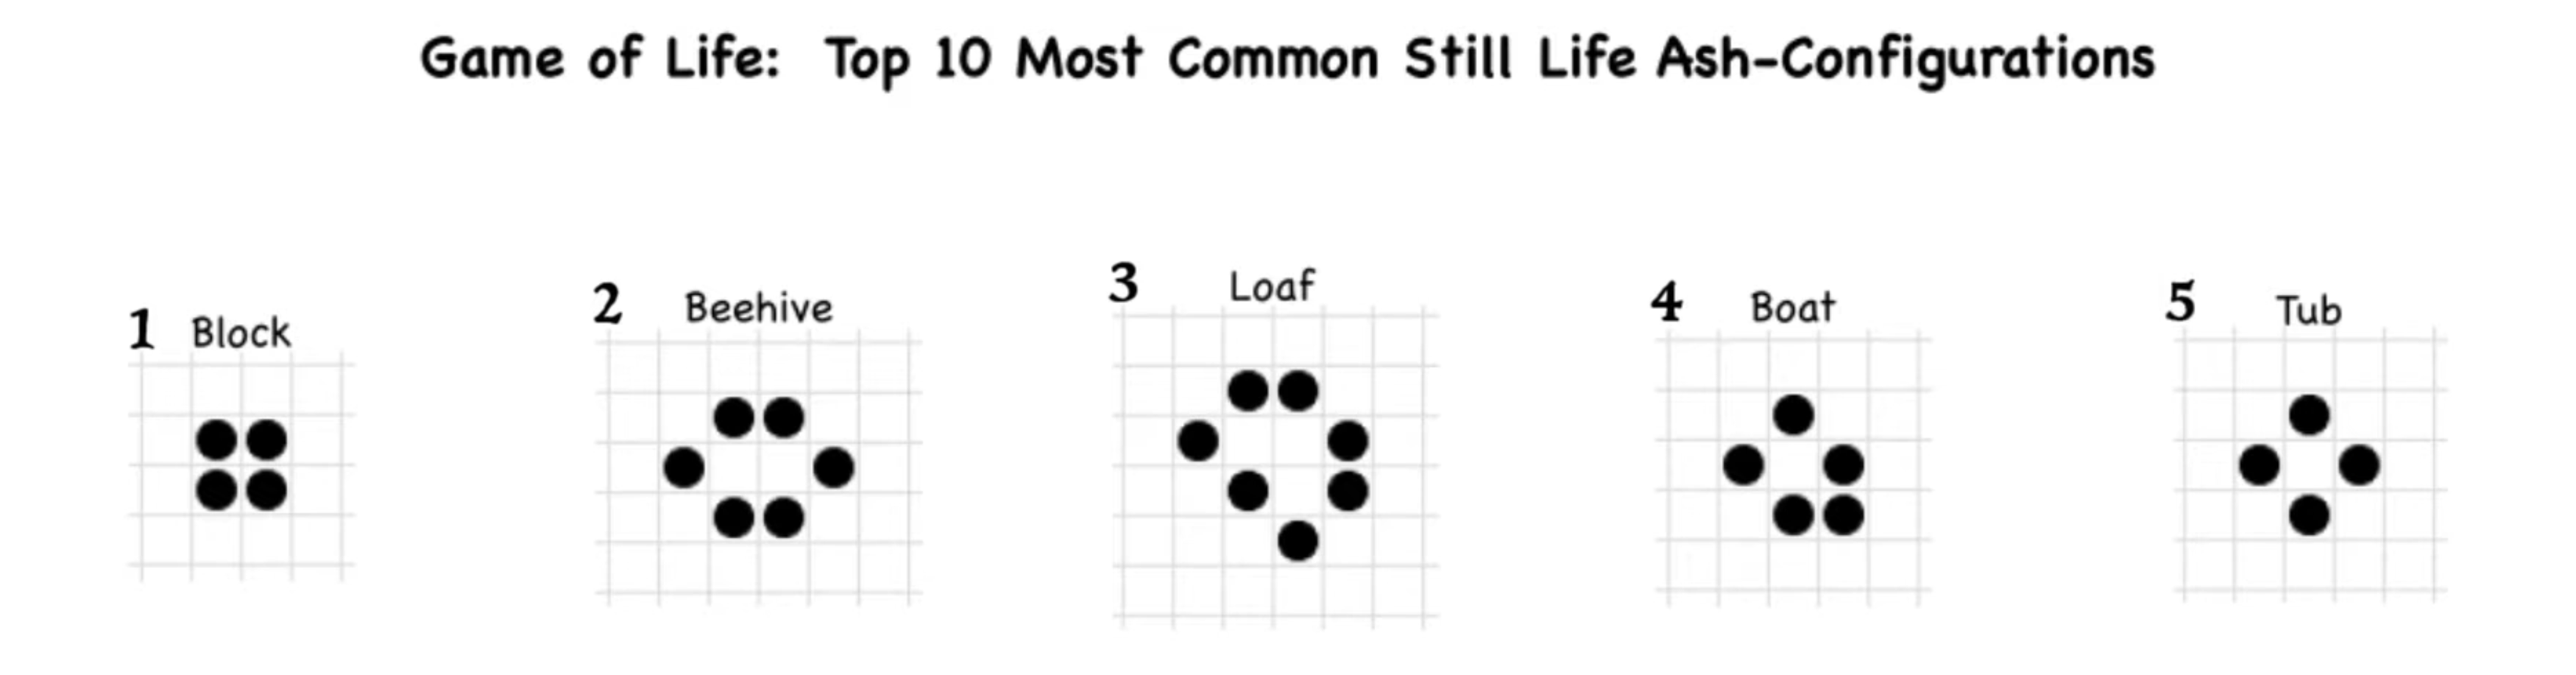
\includegraphics[width=\textwidth]{commonStillConfigurations} \\ Auflistung und Abbildung von mistercorzy \footnote{mistercorzy (Video Teil 3, bei 5:05), 2020}\\
\subsection{Der Sinn des Spiels}
	Das Spiel des Lebens ist nicht nur hübsch anzusehen, sonder dient einem festen Sinn. Laut Wikipedia haben schon viele Wissenschaftler, die sich mit zellulären Automaten auseinander gesetzt haben, den Gedanken im Hinterkopf gehabt, das dass Universum auch ein zellulärer Automat sei, der wie die Simulation, nur viel komplexer und nach viel mehr Regeln agiert\footnote{Wikipedia (Zellulärer Automat), 2020}.\\
	So lassen sich mit wenigen Regeln scheinbar komplexe Vorgänge simulieren. Das Spiel des Lebens wird dabei nicht nur unter dem biologischen Aspekt der verschiedenen Lebensformen, sonder auch den chemischen Aspekten von Energie und Materie, sowie den physikalischen Aspekten wie dem Verhalten von Kräften oder dem Anfangswertproblem betrachtet, so Wikipedia\footnote{Wikipedia (Conway's Spiel des Lebens), 2020}.
	




\newpage

\section{Quellenverzeichnis}
	Schmidt, Jörn (30.10.2014), Zellularautomaten. Letzter Zugriff: 16.01.2021, von \\https://link.springer.com/chapter/10.1007/978-3-658-01164-2\_18
	\\\\
	mistercorzi (Name auf Youtube.com) (25.08.2020 ), Conway's Game of Life (5 Parts). Letzter Zugriff: 17.01.2021, von
	\\https://www.youtube.com/playlist?list=PLvA\_gXIhzZNXdAyEGJaSA2X15-ibaXh7P
	\\\\
	Wikipedia (18.06.2020), Zellulärer Automat. Letzter Zugriff: 17.01.2021, von
	\\https://de.wikipedia.org/wiki/Zellul\%C3\%A4rer\_Automat\#Wolframs\_eindimensionales\_Universum
	\\\\
	Wikipedia (27.07.2020), Conway's Spiel des Lebens. Letzter Zugriff: 17.01.2021, von
	\\https://de.wikipedia.org/wiki/Conways\_Spiel\_des\_Lebens\#Sichtweisen
	\\\\

\newpage

\section{Anmerkung}
	Nach langem recherchieren habe ich immer noch nicht herausgefunden, warum man in der Ausgabe-PDF nicht den Character '\_' markieren bzw. kopieren kann. Dadurch ist es nicht möglich, die Links aus dem Quellenverzeichnis zu kopieren, ohne die Unterstriche im Nachhinein manuell einzufügen.

\end{document}

